\section{Impact of KID non-linearity}
\label{se:KID_NL}

\subsection{Total power}

In this paragraph we characterize KID non-linearity in total power. To do so, we simulate the observation of a point source by a KID, with a flux that we vary between \todo{1 and 2000\,Jy TBC} (fluxes are unrealistically large on purpose for illustration), to see how linear the measure remains. We assume that our instrument has a 11\,arcsec FWHM Gaussian beam like the polarized 1\,mm channel of \nikad. In the simulation, we use \methodu\ and  \methodd\ to recover the received power. We write the non linear detector response as :

\begin{equation}
m = m + \varepsilon_{det} m^2 +c_{0}.
\label{eq:model_kid_nl}
\end{equation}

\epsDET\ represents the non linearity of the KID. 
For all simulations we compute the non-linearity coefficient \epsDET\ from eq.~(\ref{eq:model_kid_nl}) by doing a linear fit of the input fluxes as a fonction of output fluxes.

Fig.~\ref{fig:planet_profiles} and Fig.~\ref{fig:flux_out_vs_in} show that under a bright source, non-linearity appears with the distortion of the input gaussian profile in the case of \methodu\ whereas \methodd\ remains linear on the same flux scale. The non-linearity coefficients that we find with \methodu\ and \methodd\ are respectively \epsDET =$-2.22 \times 10^{-5}$ and \epsDET =$8.69 \times 10^{-8}$. \todo{voir pourquoi Cf reste plus lineaire compare a Rf}.



\begin{figure}
  \includegraphics[clip, angle=0, width=\columnwidth]{Figures/planet_profiles_2.eps}
  \caption{Comparison of an incoming flux that we vary between 1 and 2000 Jy TBC (in black), with flux reconstructed by \methodu\ and \methodd. Fluxes are unrealistically large on purpose for illustration. }
  \label{fig:planet_profiles}
\end{figure}


\begin{figure}
  \includegraphics[clip, angle=0, width=\columnwidth]{Figures/flux_out_vs_in.eps}
  \caption{Comparison of an incoming flux that we vary between 1 and 2000 Jy TBC (in black), with flux reconstructed by \methodu\ and \methodd. Fluxes are unrealistically large on purpose for illustration. }
  \label{fig:flux_out_vs_in}
\end{figure}


Simulations of a KID non-linearity in total power meets the requirements (see Sec.~\ref{cmb}) necessary to not biais measures of B modes. In CMB polarization experiments, the use of Half Wave Plate to modulate polarization are more and more considered. In the next section we will study the effect that can have this signal on the KID linearity.

%In futur CMB polarization experiments, the use of a half wave plate more and more common. It presents a lot of advantages, but can also be source of various systematic effects. In the next section we will address the non-linearity that can arise from rotating a half wave plate in an instrument.

%KIDs are a novel technology successfully used in \nikad . Because of their multiplexing capability and their short time constant, they are one of the best candidates to be implemented on experiments that need larger arrays. In this section we studied KIDs non-linearity and its impact on CMB B mode measures, considering the brightness of a source, the scanning speed of the instrument and the method that we use to follow the shift of the resonant frequency and retrieve the absorbed power.
%Simulations of a KID exposed to a point source with a large variation of fluxes have shown that as expected, the brighter is the source, the more non-linearities appear due to a poor reconstruction of the resonant frequency. Although both reconstruction methods give good results, \methodd\ remains more linear at high fluxes than \methodu . Plus, KID non-linearity should not impact measures of CMB B modes, in fact the non-linearity coefficients that we found are in the range of $[10^{-5} - 10^{-8}]$, so it meets the requirement addressed in Sec.\ref{sec:cmb}.


\subsection{Polarization and Half Wave Plate}
\subsubsection{Half Wave Plate}

%\begin{itemize}
%\item les HWP deviennent a la mode
%\item les kids ont des constantes tres petites, donc on peut faire tourner vite
%  : avantages...
%\item ... mais signal parasite tres fort et donc besoin de le soustraire et de
%  voir si il n'induit pas de non linearite sur la mesure du signal
%\item simulations du HWPSS (beta): bien expliquer que ce qui compte c'est la
%  subtraction of this template not the exact recovery of the input model
%\item which constraints do we set on the HWPSS subtraction and potential
%  improvement if we could use hundreds of KIDS rather than just fit it kid by kid
%\item anticipate a bit on the achieved residual NL on the same planet as in the
%  previous section.
%\item simulate the sum of a template and pure weak signal and see the induced NL
%  on the signal
%\item comparison to NIKA(2)'s data... vs Simon's observatory perspectives
%\end{itemize}

%{\color{blue}
%Modulation of the polarization by a rotating Half Wave Plate (HWP) like in
%\nika\ and \nikad\ creates a background modulation equivalent to several tens to
%hundreds of Jy at frequencies close to the HWP rotation harmonics
%\citep{2017A&A...599A..34R}. After early tests by \todo{cite Hildebrand in the
%  80's or so ?}, this kind of modulating device has been left aside for
%\todo{20~TBC} years in the context of millimetric observations. With the
%improvement of technologies it progressively came back in the landscape, in
%particular with pioneering experiments like \emph{Maxipol}
%\citep{2007ApJ...665...42J} and \emph{EBEX} \citep{2010SPIE.7741E..1CR}. It is
%now more and more common and is considered as the leading option for future
%satellite designs such as \emph{LiteBIRD} \todo{add ref}. Such a background must
%be accounted for in the simulations.}

After early tests by \citep{1984ApJ...284L..51H}, modulation of the polarization by a rotating Half Wave Plate (HWP) has been left aside for \todo{20~TBC} years in the context of millimetric observations. With the improvement of technologies it progressively came back in the landscape, in particular with pioneering experiments like \emph{Maxipol} \citep{2007ApJ...665...42J}, \emph{SPIDER} \citep{2008SPIE.7010E..2PC}, \emph{EBEX} \citep{2010SPIE.7741E..1CR}, \emph{Polarbear} \citep{2012SPIE.8452E..1CK} \emph{BLAST-Pol} \citep{2014MNRAS.437.2772M}, \emph{ABS} \citep{2014RScI...85c9901K} and \emph{Advanced ACTPol} \citep{2016JLTP..184..772H}. It is now more and more common and is considered as the leading option for future satellite designs such as \emph{LiteBIRD} \citep{2014JLTP..176..733M} and next generation ground based experiments such as \emph{CMB-S4} \citep{2016arXiv161002743A}. The rotation of the HWP can be stepped (\emph{POLARBEAR} \citep{2014ApJ...794..171P}) or continuous  (\emph{EBEX}, \emph{ABS} and \nikad\  \citep{2015fers.confE..16R}).
Using a HWP to modulate the polarization is a powerful tool to mitigate several instrumental systematics \citep{2009MNRAS.397..634B}. In fact, with a HWP :

\begin{itemize}
\item The polarized signal is modulated at 4 times the rotation frequency of the HWP and therefore is shifted at higher frequencies, isolating it from electronic noise and 1/f noise. This is valid if the rotation of the HWP is continous and fast ( HWP rotation frequency of \emph{EBEX} and \nika\ are respectively 1.235 Hz \citep{2018ApJS..239....7T} and 2.98 Hz \citep{2017A&A...599A..34R}.)

\item A single detector $k$ can measure a combination of the three Stokes parameters $I$, $Q$ and $U$ :

\begin{equation}
\label{eq:polar_measure}
m_{k}(t) = \frac{1}{2} [I + \rho [Q \cos (4 \omega t + 2 \alpha(t)) + U \sin (4 \omega t + 2 \alpha(t))]],
\end{equation}

with $\alpha$ the angle between the telescope reference frame and the local meridian on the sky and $\omega t$ is the position angle of the HWP.
This allows to do observations without having to use differencing polarization sensitive detectors and thus avoid systematic effects such as intensity to polarization leakage from mismatch of the detector beams.

\item We can achieve an optimal angular coverage as each pixel will be observed over a wide range of orientations. This allows to have a better angular redundancy in a single pixel to measure the Stokes parameters without having to rotate the full instrument.
\end{itemize}

On the down side, rotating a HWP can also be source of several systematic effects like : mis-estimation of the HWP angles, leakage of temperature into polarization due imperfection in the optical system, differential transmittance in the HWP \citep{2009MNRAS.397..634B,2018SPIE10708E..48S} and the introduction of a strong parasitic signal that is synchronous with the HWP rotation. It is on the latter that we focus in this paper.

\subsection{Half Wave Plate Synchronous Signal}

Modulation of the polarization by a rotating HWP like in \nika\ and \nikad\ creates a background modulation equivalent to several tens to hundreds of Jy at frequencies close to the HWP rotation harmonics \citep{2017A&A...599A..34R} (see Fig. \ref{fig:hwp_power_spectrum}).

\begin{figure}[h]
\center
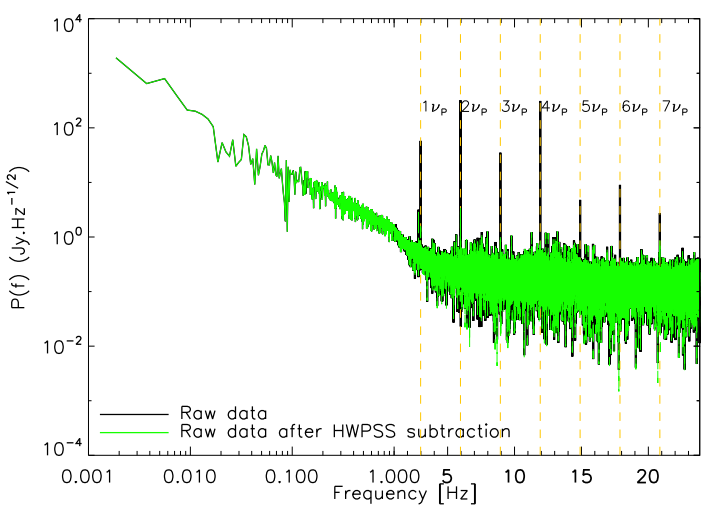
\includegraphics[clip, angle=0, width=\columnwidth]{Figures/hwp_power_spectrum.png}
\caption{Power spectrum of an observation of Orion OMC-1 for one KID. The observations were done with \nika . Black and green lines represent respectively the raw data and the raw data after subtraction of the HWP parasitic signal. Credits : \citet{2017A&A...599A..34R} }
\label{fig:hwp_power_spectrum}
\end{figure}

This additional parasitic signal was observed by experiments like \nika2\ , \emph{EBEX} \citep{2010SPIE.7741E..1CR} and \emph{MAXIPOL} \citep{2007ApJ...665...42J}. This Half Wave Plate Synchronous Signal (HWPSS) can be modelled by a sum of $n$ harmonics of the HWP rotation frequency $\nu_{p}$ with amplitudes $A_{n}$ and $B_{n}$ that are linearly drifting :

\begin{equation}
HWPSS(t) = \sum_{n=1} A_{n} \cos nwt + B_{n} \sin nwt , 
\label{eq:hwp-template}
\end{equation}

where : 
\begin{eqnarray}
A_{n}  &=& A_{n}^{0} + \varepsilon_{A_{n}}t,\\
B_{n}  &=& B_{n}^{0} + \varepsilon_{B_{n}}t, 
\end{eqnarray}

with $w = 2 \pi \nu_{p}$.
This effect can then be corrected by subtracting observations by the model presented in eq.~\ref{eq:hwp-template}. 

A large amplitude of the HWPSS can cause non-linearity in the detector response. This non-linear response can then be the source of coupling between intensity and polarization signals. Systematic effects arising from detector non-linearity have been studied in \emph{Simon's Observatory} \citep{2018SPIE10708E..48S}, \emph{POLARBEAR} \citep{2017JCAP...05..008T} and \emph{EBEX} \citep{2017arXiv171101314D}. In the latter, it was shown that the dominant source of intensity to polarization leakage is due to detector non-linearity caused by a large HWPSS. 

In \nikad\ this additionnal noise is two to three order of magnitude above the noise level, making it one of the strongest noise contributor in polarization observations, such a bakground must be accounted for in the simulations. In the next paragraph, we study the non-linearity of a KID caused by a large HWPSS. 


\subsection{Simulations}

To account for the HWPSS we keep the instrumental parameters of Sect.~\ref{se:kids} and we simulate the observation of a point source, with a flux that varies between 1 and 500 Jy, plus the signal corresponding to HWPSS with a maximum amplitude of 70 Jy. We suppose that the subtraction of the HWPSS template is perfect. Fig.~\ref{fig:histos_epsilon_rf} and Fig.~\ref{fig:histos_epsilon_cf} show the distribution of non-linearity coefficients for different scanning speed and different method of signal reconstruction (\rf\ and \cf). 

\begin{figure}
	\includegraphics[clip, angle=0, width=\columnwidth]{Figures/histos_epsilon_rf.eps}
	\caption{histogram of non-linearity coefficients derived with \rf\ and scanning speed equal to 3 and 5 points per beam.}
	\label{fig:histos_epsilon_rf}
\end{figure}

\begin{figure}
	\includegraphics[clip, angle=0, width=\columnwidth]{Figures/histos_epsilon_cf.eps}
	\caption{histogram of non-linearity coefficients derived with \cf\ and scanning speed equal to 3 and 5 points per beam.}
	\label{fig:histos_epsilon_cf}
\end{figure}

The average of the non-linearity coefficients are given Tab.~\ref{tab:eps_hwp}, where we can see that on the same flux scale, \cf\ remains more linear than \rf . The non-linearity coefficients derived from the simulations are lower than the non-linearity coefficient required in Sect.~\ref{sec:cmb} to detect B modes without being biaised by non-linearity arising from the detector and the HWPSS. 

\begin{table}
\center
\begin{tabular}{|c|c|c|}
	\hline
	    & $\frac{3pts}{beam}$ & $\frac{5pts}{beam}$ \\
	\hline
\rf\	&  $-4.8 \times 10^{-5}$ & $-2.4 \times 10^{-5}$ \\
	\hline
\cf\ & $-6.6 \times 10^{-7}$ & $-5.4 \times 10^{-7}$ \\
	\hline
\end{tabular}
\caption{Non-linearity coefficients $\varepsilon$ from an incoming flux that we vary between 1 and 500 Jy.}
\label{tab:eps_hwp}
\end{table}




\subsubsection{Simulations}





